\documentclass{article}

% if you need to pass options to natbib, use, e.g.:
%     \PassOptionsToPackage{numbers, compress}{natbib}
% before loading neurips_2021

% ready for submission
\usepackage[preprint]{neurips_2021}
\usepackage{graphicx}

% to compile a preprint version, e.g., for submission to arXiv, add add the
% [preprint] option:
%     \usepackage[preprint]{neurips_2021}

% to compile a camera-ready version, add the [final] option, e.g.:
%     \usepackage[final]{neurips_2021}

% to avoid loading the natbib package, add option nonatbib:
%    \usepackage[nonatbib]{neurips_2021}

\usepackage[utf8]{inputenc} % allow utf-8 input
\usepackage[T1]{fontenc}    % use 8-bit T1 fonts
\usepackage[colorlinks=true]{hyperref}       % hyperlinks
\usepackage{url}            % simple URL typesetting
\usepackage{booktabs}       % professional-quality tables
\usepackage{amsfonts}       % blackboard math symbols
\usepackage{nicefrac}       % compact symbols for 1/2, etc.
\usepackage{microtype}      % microtypography
\usepackage{xcolor}         % colors

\title{Toward an understanding of salary distributions in remote workers}

% The \author macro works with any number of authors. There are two commands
% used to separate the names and addresses of multiple authors: \And and \AND.
%
% Using \And between authors leaves it to LaTeX to determine where to break the
% lines. Using \AND forces a line break at that point. So, if LaTeX puts 3 of 4
% authors names on the first line, and the last on the second line, try using
% \AND instead of \And before the third author name.

\author{%
  Tim Schreier\\
  Matrikelnummer: 5634978\\
  \texttt{tim.schreier@student.uni-tuebingen.de} \\
  \And
  Luca Schaal\\
  Matrikelnummer: 6052577\\
  \texttt{luca.schaal@student.uni-tuebingen.de} \\
}

\begin{document}

\maketitle

\begin{abstract}
Our project\footnote{Link to the relevant  \href{https://github.com/Lucahalt/Data-Literacy-Final-Project
}{Git-repository}}
revolved around this  \href{https://salaries.freshremote.work/download/}{data set of characteristics of global remote worker}. 
After an examination of the data source itself, we continued to inspect the data critically and thus discuss the data set and its limitations for our investigation in the first paragraph of this report. 
We then continued to inspect the data and found various patters relevant for salary distributions. For the most insightful of these, we included visualizations in this report.
We furthermore investigated our hypotheses that the mean salaries between fully remote jobs and jobs that are only partly remote differ significantly using a standard t-test for independent samples.

\end{abstract}
\section{The data set and its limitations}
\label{sec:dataset}
At the time of our analysis, the data set of global remote work salaries, contained 1507 entries. It includes salary data from professionals around the world in the field of remote work. There are various features, such as experience level, employment type, company size, company location and remote ratio. The data set includes the salary in local currency as well as converted into US dollars, for comparability we always use the salary in USD in the following. The data set is regularly expanded and the data contained therein is collected on a voluntary basis, via an input form. For this reason, there is no official source that verifies this data. 

Moreover, many different jobs are included in the data set, executives are compared with ordinary workers, which leads to large differences in salary. Since the job descriptions are contained in plain text in the data set, it is difficult to filter or group them. This fact must be taken into account when reading our analysis. There are also job descriptions, which have a similar meaning, e.g. ML Engineer and Machine Learning Engineer. 

Looking at the residence of employees, we find that nearly half of all employees are from the U.S. (49.9\%). In addition, there are countries from which there are no data at all (indicated by the gray countries in \autoref{fig:world_data}). This makes generalized inferences difficult since the data is so strongly biased toward residence of the USA.

\begin{figure}
\centering
\caption{Number of employees per country (no data for gray countries)}
\label{fig:world_data}
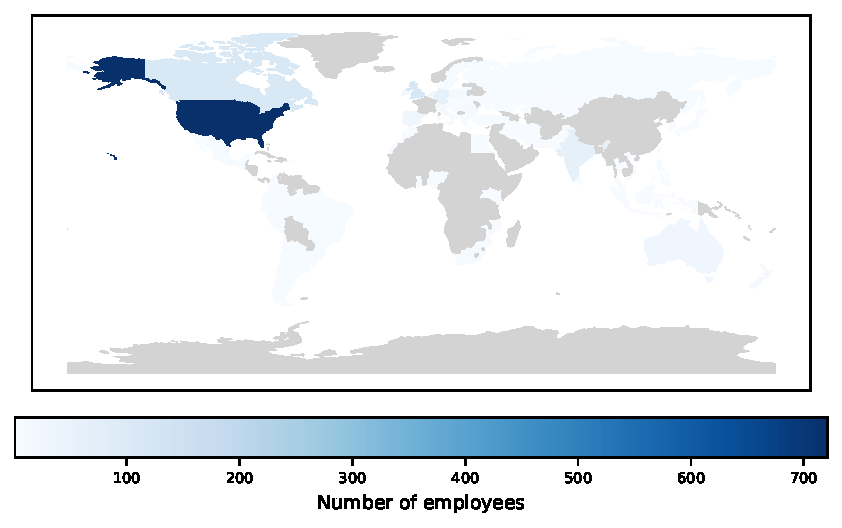
\includegraphics[scale=0.85]{fig/world_employee_residence.pdf}
\end{figure}

At the beginning, we were interested in finding out what the impact on salary is when you work at a U.S. company but live somewhere else. However, the data shed little light on this question, since almost all workers who work for U.S. companies also live there (88.6\%).

\section{Understanding the data}
To get a more detailed overview of the data and to better understand the distributions, we did several visual inspections. 

Firstly, we looked at the average salary per country, based on the company location. It should be noted that for some countries there is exactly one entry, which distorts the data. When looking at this, we have already filtered out large outliers for this reason. In addition, as mentioned in \autoref{sec:dataset}, the data set does not contain data for every country (the gray-colored countries in \autoref{fig:world_data_2} do not contain any data). As can be seen by looking at the figure, there are still outliers, for example in Iraq. Nevertheless, it can be said that one earns relatively much in the USA as well as in Australia and Canada. However, it is important to keep in mind that there are very different kinds of jobs and experience levels contained in the data. This plot alone is thus not sufficient to rank countries by their average salary.

\begin{figure}[h]
\centering
\caption{Average salary per per country (no data for gray countries)}
\label{fig:world_data_2}
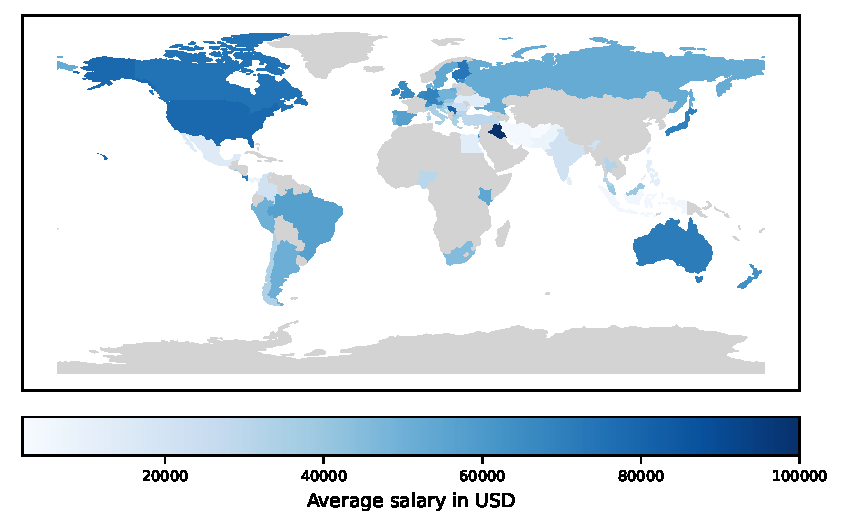
\includegraphics[scale=0.85]{fig/world_salary_company_location.pdf}
\end{figure}

For this reason, in the next step we will look at the impact of experience level and company size on salary. For this purpose, we have created a boxenplot (\autoref{fig:boxplot}) which distinguishes the company size by color and the experience levels on the X-axis. It can be clearly seen that the salary increases with both the size of the company and the level of experience.

However, these data must also be treated with caution, as there is an imbalance in the data between the different experience levels. %vielleicht noch einen Prozentsatz oder Zahlen als veranschaulichung des unterschieds

\begin{figure}[h]
\centering
\caption{Salary cataloged by company size and experience level}
\label{fig:boxplot}
\hspace*{-0.55cm}
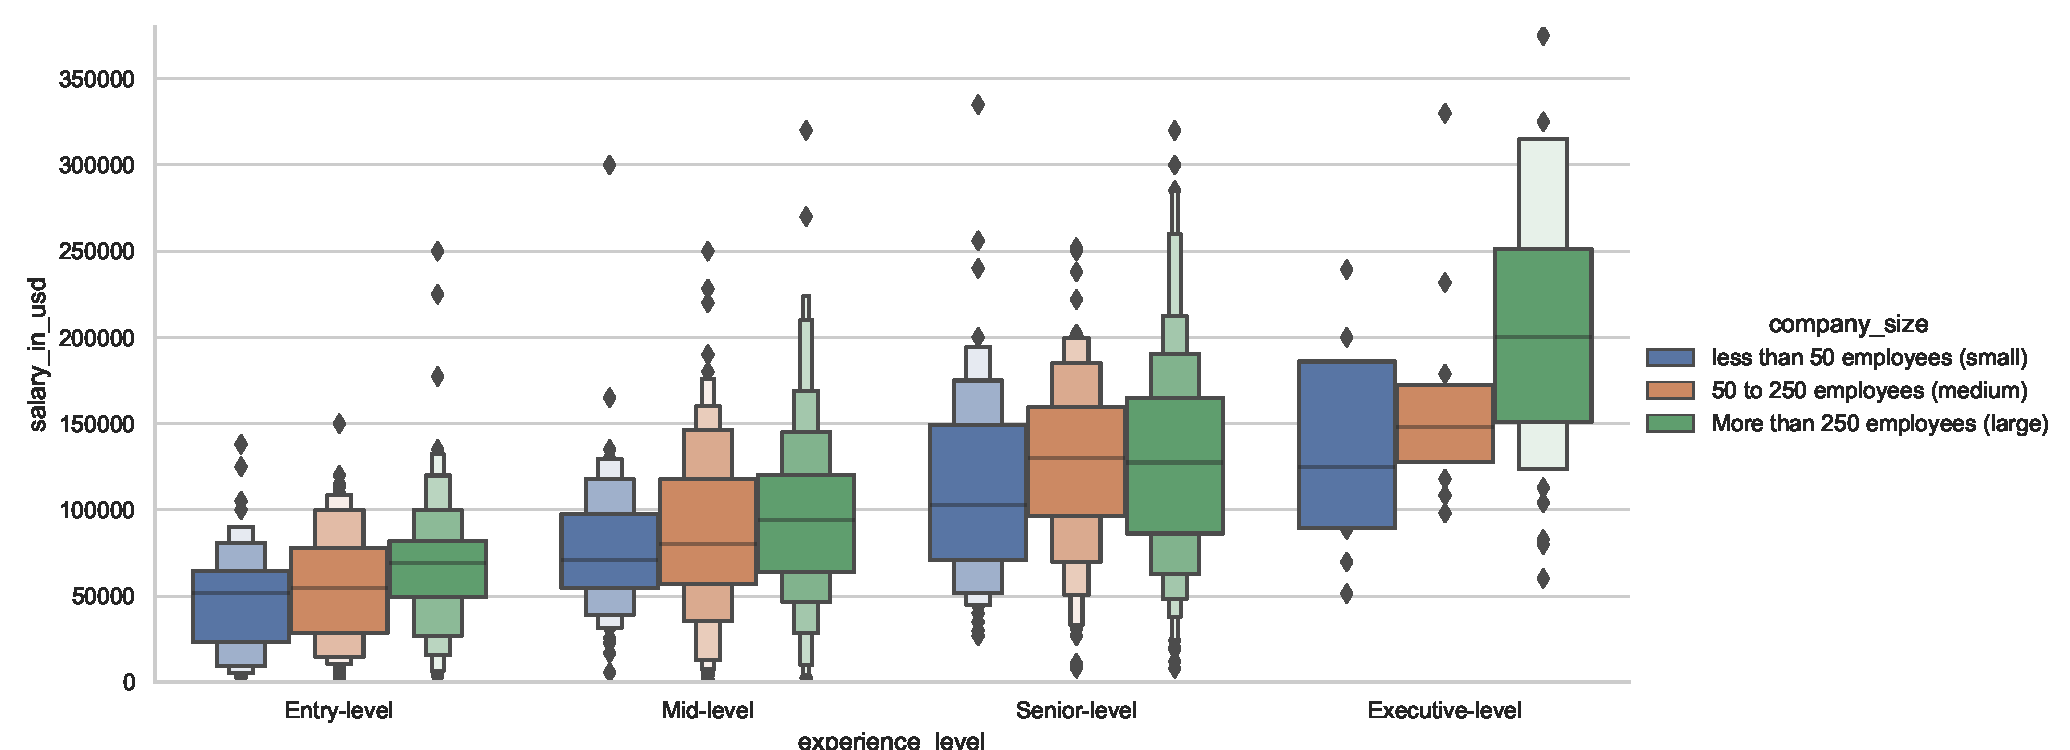
\includegraphics[scale=0.5]{fig/experience_level.pdf}
\end{figure}



\section{Testing our hypothesis}

In this part of our analysis we investigate whether people that work 100\% remote earn significantly more or less money on average compared to those that only partly work remotely.

Since we are trying to compare the mean values of two independent groups, we are going to use the standard t-test for independent samples. Our null-hypotheses is that both groups earn the same amount of money on average, so we are going to use a two-sided test to test for deviations in both directions.

Since our data is very heterogeneous, we only consider data points from people who live in the USA, work full-time and hold entry level positions. We then considered the groups to be homogeneous enough to compare them. One obvious caveat is that the very category of 'remote jobs' spans a wide range of job descriptions, each of which has a different average income, but we decided to proceed various job titles in both groups for a lack of sufficient data.

As a next step we take a look at the filtered data. In \autoref{fig:incomes_remote_levels} we can make a couple of observations. First of all, that the two classes are not balanced. There are 82 samples in the fully remote group but only 38 in the partly remote group. But this is not problematic for the standard t-test. The second observation is that there are outliers in the data. These could significantly skew the results of the test and we hence decide to exclude them from our analysis.

\begin{figure}[!htb]
\centering
\caption{Comparing incomes across groups}
\label{fig:incomes_remote_levels}
\hspace*{-1.2cm}   
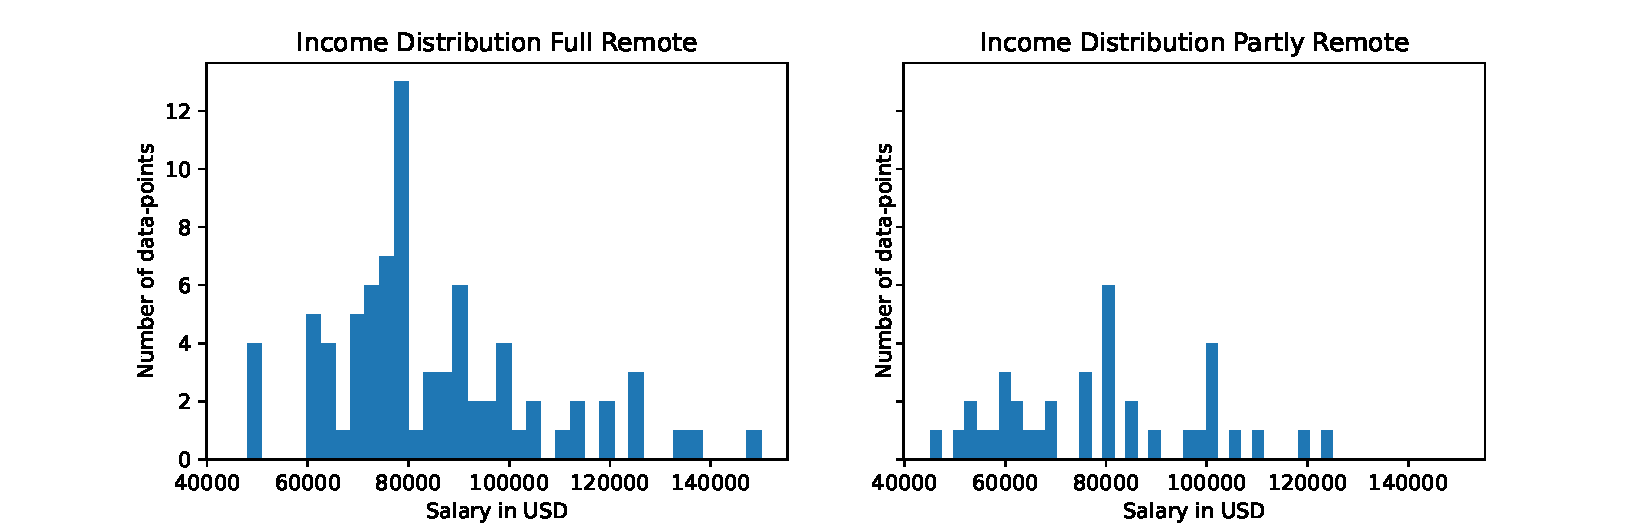
\includegraphics[scale=0.55]{fig/incomes_remote_levels.pdf}
\end{figure}

So our null-hypotheses is that there is no difference between the salaries of jobs that are fully remote and the ones that are only partly remote. We want to test if the data provides us with a reason to question this hypotheses. Before the test, we decide on a significance level of $\alpha=5\%$  
, which will only reject the null hypotheses by accident in one out of twenty cases. 

Before computing the test statistic, we have to firstly check if the assumptions for the standard t-test with two independent samples apply. The first assumption states that the samples must be independent from each other. Since our data is not paired in any way, we assume this to be true. 

The second assumption states that the samples must come from a random sample of a population. This is definitely not the case if we regard all remote workers (in the USA) as the population we are concerning ourselves with. Our data should rather be regarded as a convenience sample of the population of remote workers that has been created by the process described in \autoref{sec:dataset} (which does not constitute a random sample). We could sidestep this by defining only the samples present in our data set as the total population, but this would then prevent us from making inferences beyond the samples present in the data set. 

A third assumption of the t-test is about homogeneity of variances. It states that both groups should have the same intra-group variance. A quick check of the standard variations reveals that this assumption seems to be satisfied. 
$$\sigma(partly\_remote)=19998 \hspace{1cm} \sigma(full\_remote)=20902$$

The forth and last assumption is that of normality. A quick look at  \autoref{fig:incomes_remote_levels} indicates that especially the distribution of the partly-remote group does not look a lot like the Gaussian bell-curve, but we will test for normality using a visual inspection via quantil-quantil plot against the normal-distribution.  \autoref{fig:QQ} demonstrates that even though the empirical distributions are fairly similar to the normal distribution, there are systematic deviations from the line of comparison, which undermine the assumption of normality. Since we are dealing with relativly small sample sizes, we still decided to continue, being aware that these deviations from the normality assumption might influence our results.

\begin{figure}[!htb]
\begin{center}
\caption{Testing the distributions for normality}
\label{fig:QQ}
\hspace*{-1.3cm}   
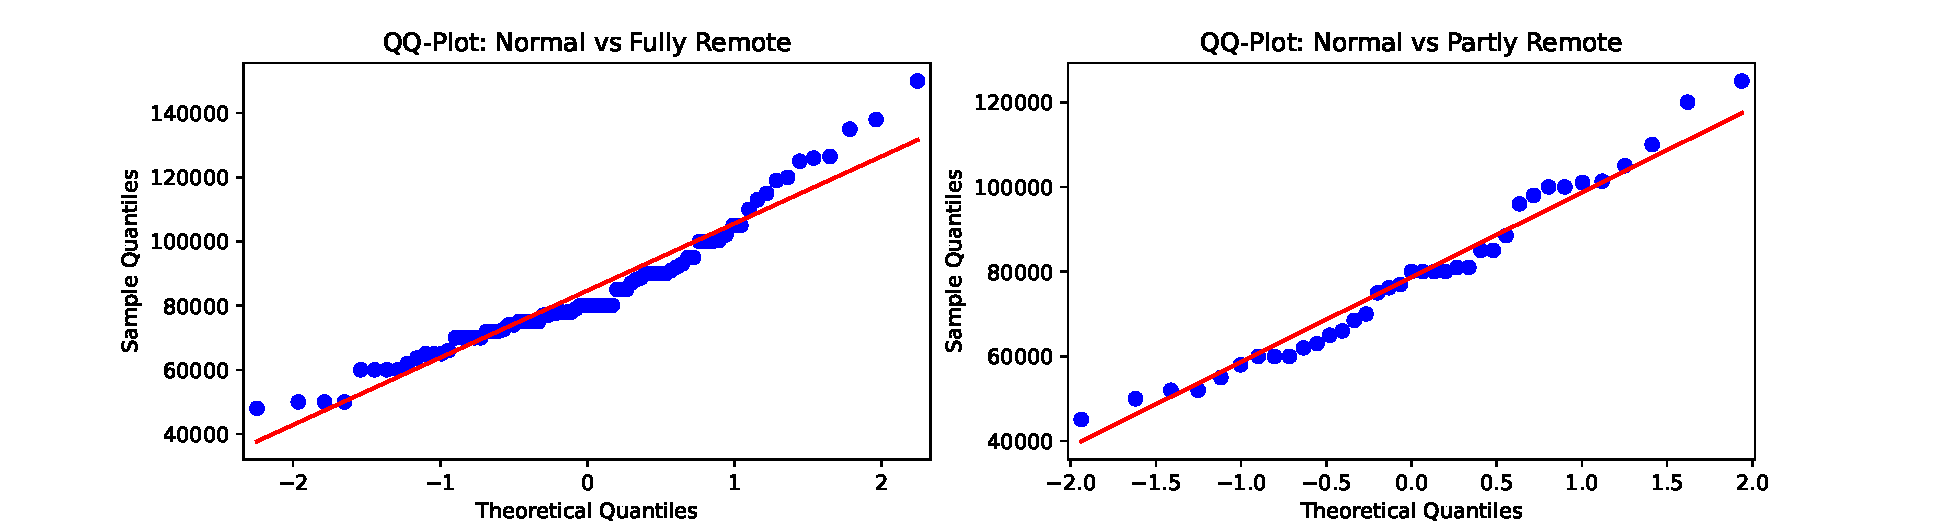
\includegraphics[scale=0.52]{fig/QQ.pdf}
\end{center}
\end{figure}


Having cast sufficient doubt on the applicability of t-test in this scenario, we finally do the calculations and arrive at the following p-value = 0.1519. 
We can thus conclude our report with the insight that we should not reject the (null-) hypotheses that full-time full-remote workers holding entry level positions in the USA earn differently on average compared to their half-remote working counterparts. 


\end{document}
